\documentclass[dvipdfmx]{jsarticle}

\usepackage[version=3]{mhchem}
\usepackage{amsmath}
\usepackage[siunitx]{circuitikz}
\usepackage{graphicx}
\usepackage{here}

\setlength\parindent{0pt}

\begin{document}
\title{16 半導体デバイスキャリア統計と電子輸送現象  総合報告書}
\author{電子情報工学科 03-190449 堀 紡希}
\date{\ 10月21日}
\maketitle


\section{抄録}
半導体のキャリアの振る舞いを、代表的なデバイスにおける電子電動現象とホール効果の測定を通じて体感することで、半導体物性と電子デバイスについて理解する。
\section{目的}
半導体のキャリアの振る舞いを、代表的なデバイスにおける電子電動現象とホール効果の測定を通じて体感することで、半導体物性と電子デバイスについて理解する。実験結果を理論と比較検討することにより、半導体のキャリア統計と電子伝導の現象の基礎を学ぶ。
\section{実験}

\subsection{原理}
ホール効果の概要を図1に示す。
\begin{figure}[H]
\begin{center}
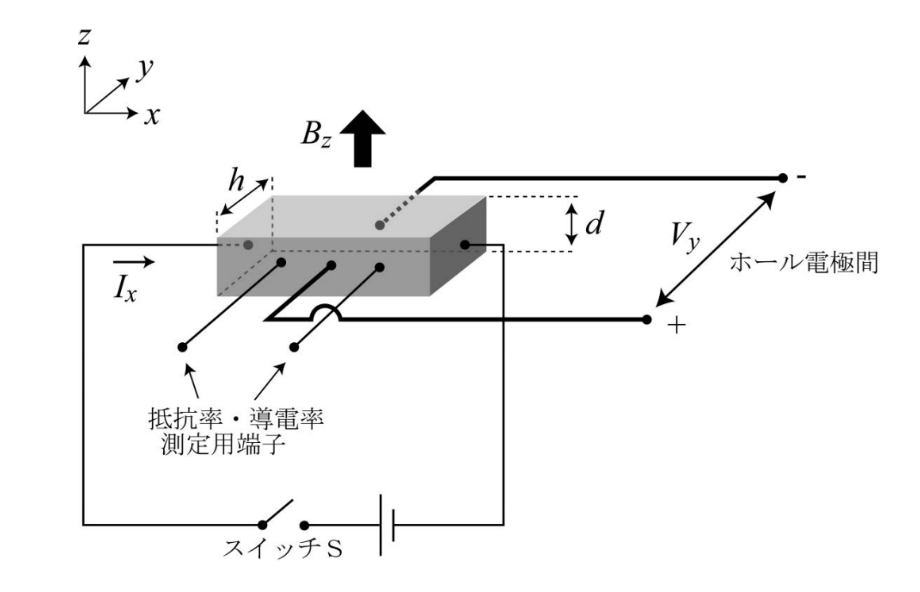
\includegraphics[scale = 0.6]{figure1.png}
\caption{ホール効果の測定}
\end{center}
\end{figure}

図のように$x,y,z$軸をそれぞれ定めると、厚さ$d$(m)の試料に電流$I_{x}$(A),磁束密度$B_{z}$(T)をかけたとき、ホール電圧$V_{y}$(V)が
\begin{equation}
V_{y} = R_{H}\frac{I_{x}B_{z}}{d}
\end{equation}
生じる。ここで$R_{H}$は試料によって定まるホール係数である。

図1において、試料がp型半導体と仮定して、ドリフト速度$v_{x}$で移動すると仮定すると正孔が受けるローレンツ力は正孔の電荷を$q$として、
\begin{equation}
F_{y} = -qv_{x}B_{z}
\end{equation}
と表される。
定常状態において、ローレンツ力と、密度勾配によって生じる電界が釣り合うので、$qE_{y} = qv_{x}B_{z}$が成り立つから、正孔の密度をp[1/cm$^{3}$]とすると、$I_{x} = pqv_{x}hd$より
\begin{align}
V_{y} &= E_{y}h\\
&= v_{x}B_{z}h\\
&= \frac{1}{pq}\frac{I_{x}B_{z}}{d}
\end{align}
となる。
(1)と比較して、
\begin{equation}
R_{H} = \frac{1}{pq}
\end{equation}
である。

n型の場合は、$p = -n$とすればそのまま成り立つ。

しかし、本実験では半導体がボルツマン分布に従い、電子や正孔が熱散乱を受けると考え、
\begin{equation}
R_{H} = \frac{3\pi}{8pq}, -\frac{3\pi}{8nq}
\end{equation}
とする。

ホール効果の測定から測定試料のキャリア濃度と移動度を求めるために、パウ法(後述)で電導率$\sigma$を求め、p型半導体の場合は、
\begin{equation}
p = \frac{3 \pi }{8}\frac{1}{qR_{H}}
\end{equation}
\begin{equation}
\mu _{p} = \frac{8}{3 \pi} \sigma R_{H}
\end{equation}
と求められる。(n型も同様)


次にパウ法によって試料の抵抗率、ホール係数を測定する方法を紹介する。
\begin{figure}[H]
\begin{center}
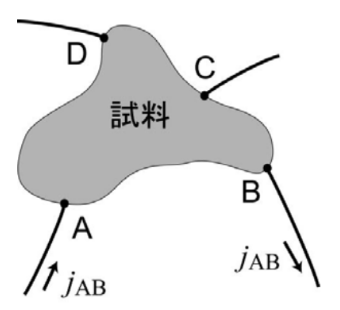
\includegraphics[scale = 0.6]{figure2.png}
\caption{パウ法による測定}
\end{center}
\end{figure}
試料の厚さが均一のとき、図2のようにサイクリックに電極を配置し(電極の位置は任意)電極Aから電極Bに電流$j_{AB}$を流したときに、電極C,D間に生じる電位差を$V_{D}-V_{C}$とする。$R_{\rm{AB} \cdot \rm{CD}}$を
\begin{equation}
R_{\rm{AB} \cdot \rm{CD}} = \frac{V_{D}-V_{C}}{j_{AB}}
\end{equation}
と定義すると、抵抗率$\rho$は
\begin{equation}
\rho = \frac{\pi d}{\rm{ln}2}\frac{R_{\rm{AB} \cdot \rm{CD}} + R_{\rm{BC} \cdot \rm{DA}}}{2}f\left(\frac{R_{\rm{AB} \cdot \rm{CD}}}{R_{\rm{BC} \cdot \rm{DA}}}\right)
\end{equation}
と表せる。
ただし$f$は
\begin{equation}
\frac{R_{\rm{AB} \cdot \rm{CD}} + R_{\rm{BC} \cdot \rm{DA}}}{R_{\rm{AB} \cdot \rm{CD}} - R_{\rm{BC} \cdot \rm{DA}}} = \frac{f}{\rm{ln}2}\left(\cosh^{-1}\frac{exp(\rm{ln}2/f)}{2}\right)
\end{equation}
を満たす。


またホール係数は試料に垂直に磁場Bをかけたときの$R_{AC\cdot BD}$の変化を$\Delta R_{\rm{AC}\cdot \rm{BD}}$とすると、
\begin{equation}
R_{\rm{H}} = \frac{d}{B}\cdot \Delta R_{\rm{AC}\cdot \rm{BD}}
\end{equation}
移動度は
\begin{equation}
\mu = \frac{d}{B}\cdot \frac{\Delta R_{\rm{AC}\cdot \rm{BD}}}{\rho}
\end{equation}
と表される。
\subsection{方法}
\subsubsection{実験(1) 室温}
実験班5人の中で2グループに分かれ、Ge, 厚さが異なるSi, GaAs試料のそれぞれについて、電流$I_{\rm{x}}$を流し、室温における導電率をパウ法を使って求め、次に磁場$B_{\rm{z}}$を変化させながらかけて、ホール電圧を測定することでホール係数を求め、さらにそこから、キャリア密度、ホール移動度計算する。

また、ホール係数の符号から試料の導電型を判定する。


\subsubsection{実験(2) 温度変化}
室温で行った実験をクライオスタット、液体窒素を用いて温度を変えながら行うことで、移動度、キャリア密度の変化を求める。

具体的には-196℃から0℃まで7点、30℃から130℃まで7点測定する。


\subsubsection{実験 異常ホール効果}

強磁性半導体であるGaMnAsを4Kから100Kまでの間で-500Gから500Gの磁場の間でホール効果を測定することで異常ホール効果を観測する。

なお本実験はプログラムを用いて測定する。
\section{結果}

\begin{figure}[H]
\begin{center}
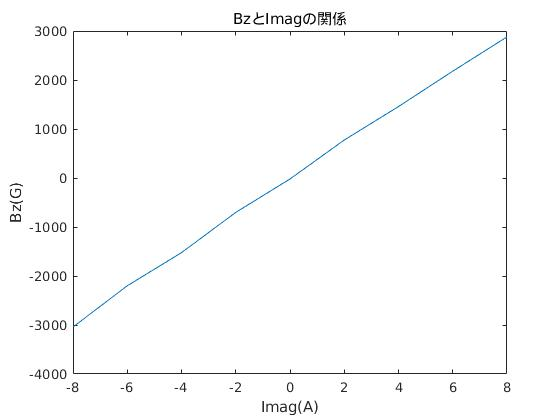
\includegraphics[scale = 0.7]{ImagBz.jpg}
\caption{$B_{z}$と$I_{mag}$の関係}
\end{center}
\end{figure}

図3は$B_{z}$と$I_{mag}$の関係であり、予想通り、$B_{z}$が$I_{mag}$に比例している。

\newpage
以下は各試料のホール効果特性である。縦軸にホール電圧、横軸に$I_{x}B_{z}/d$をとることで、式(1)からこれらのグラフの傾きがホール係数になる。

\begin{figure}[H]
\begin{center}
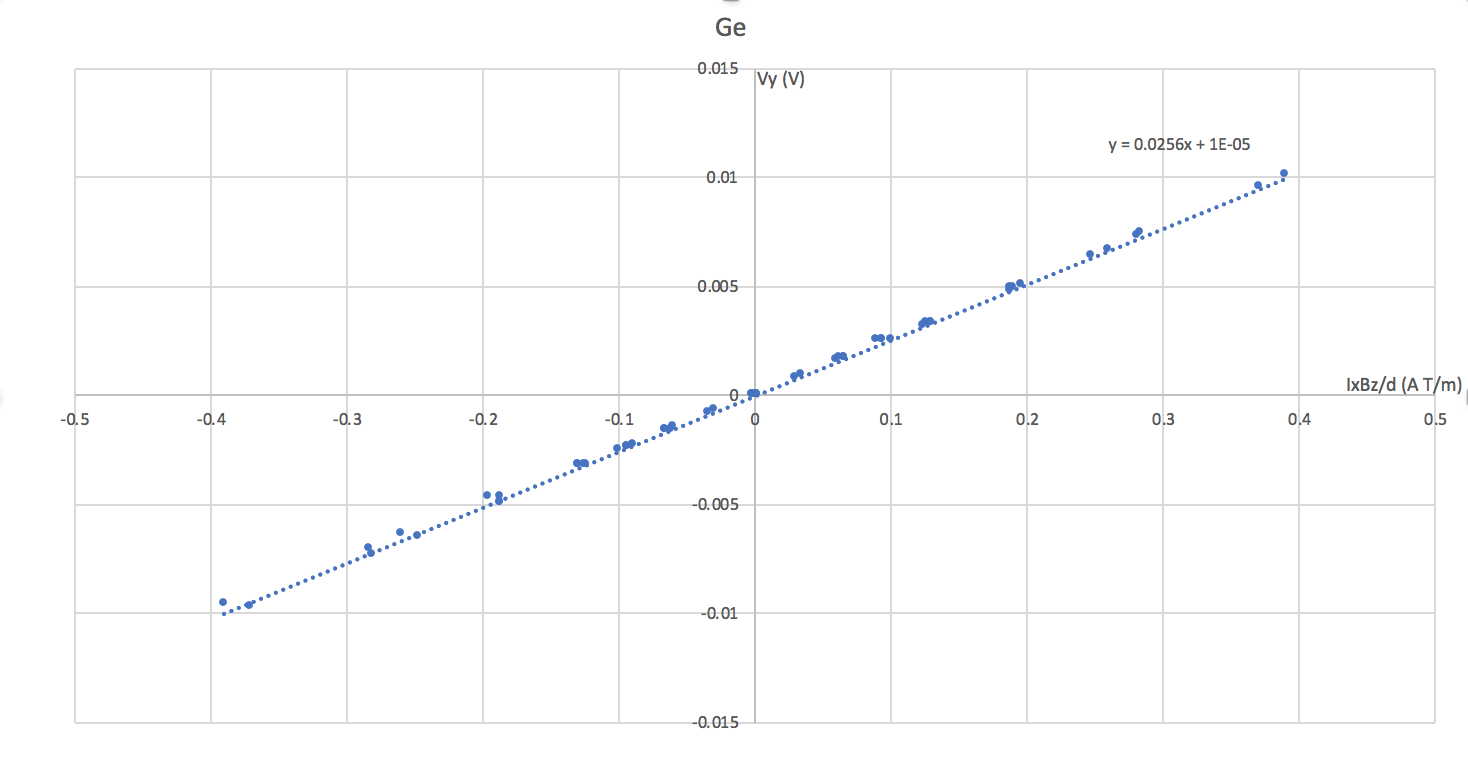
\includegraphics[scale = 0.6]{Ge.png}
\caption{Ge試料のホール効果特性}
\end{center}
\end{figure}

\begin{figure}[H]
\begin{center}
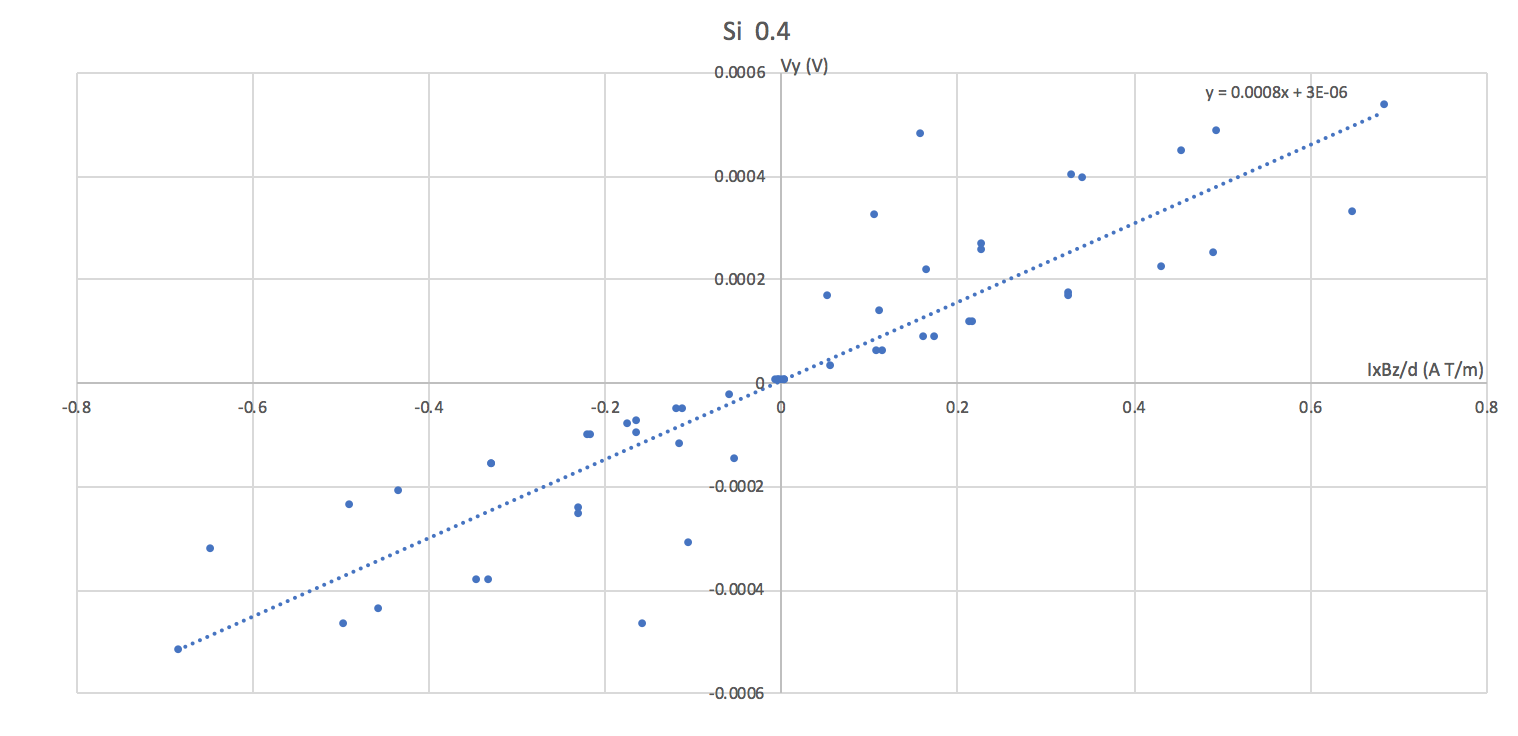
\includegraphics[scale = 0.6]{Si04.png}
\caption{Si試料(0.4mm)のホール効果特性}
\end{center}
\end{figure}

\begin{figure}[H]
\begin{center}
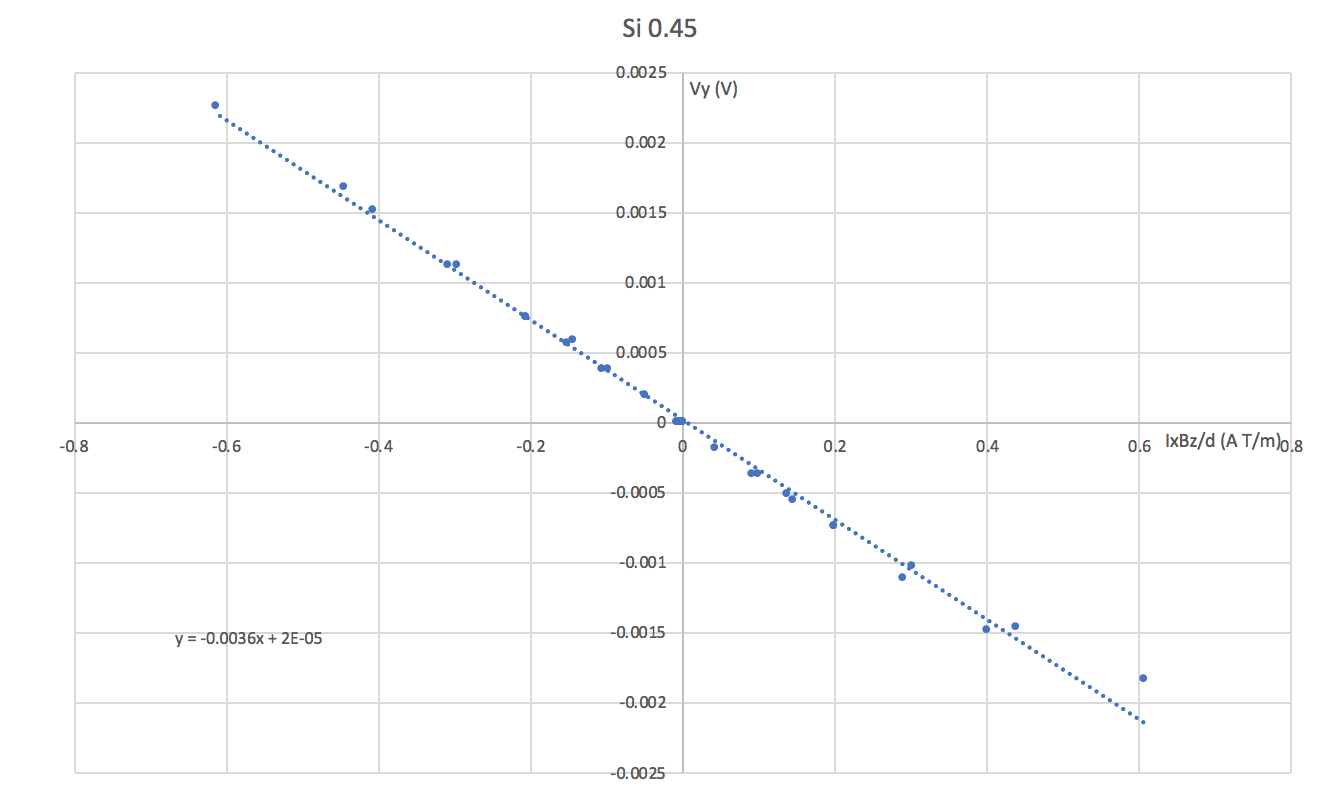
\includegraphics[scale = 0.6]{GaAs6.png}
\caption{Si試料(0.45mm)のホール効果特性}
\end{center}
\end{figure}

\begin{figure}[H]
\begin{center}
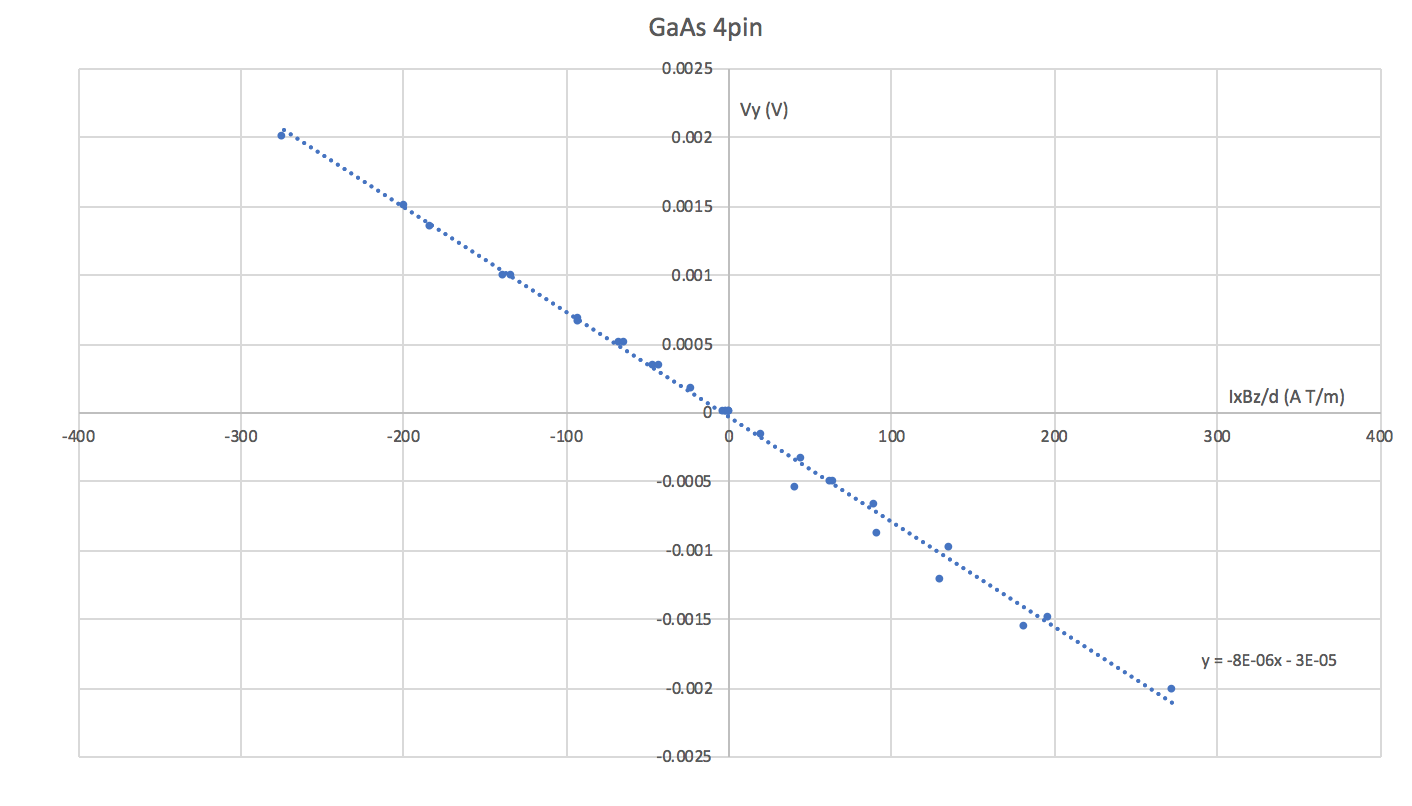
\includegraphics[scale = 0.6]{GaAs4.png}
\caption{GaAs試料(4ピン)のホール効果特性}
\end{center}
\end{figure}

\begin{figure}[H]
\begin{center}
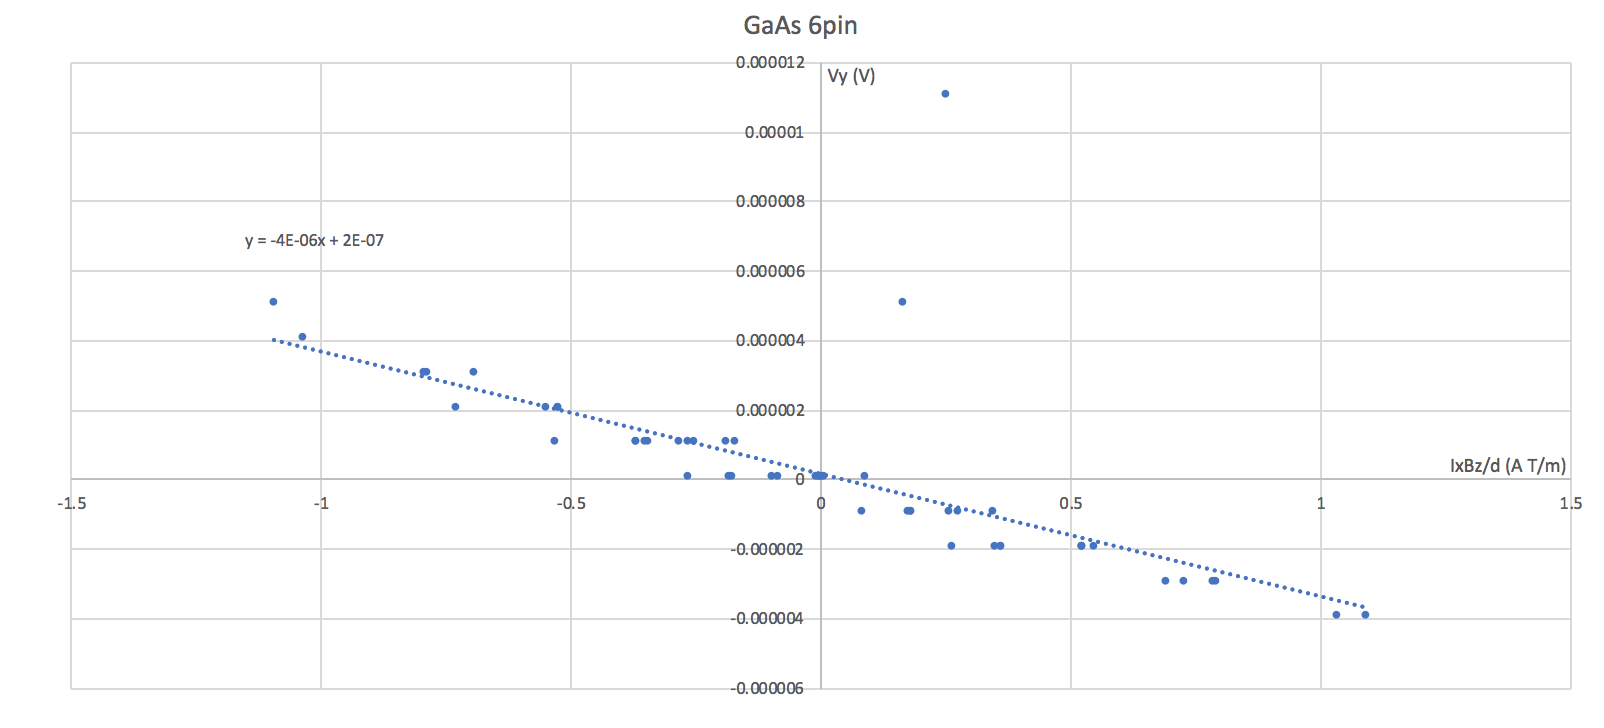
\includegraphics[scale = 0.6]{Si045.png}
\caption{GaAs試料(6ピン)のホール効果特性}
\end{center}
\end{figure}


\begin{figure}[H]
\begin{center}
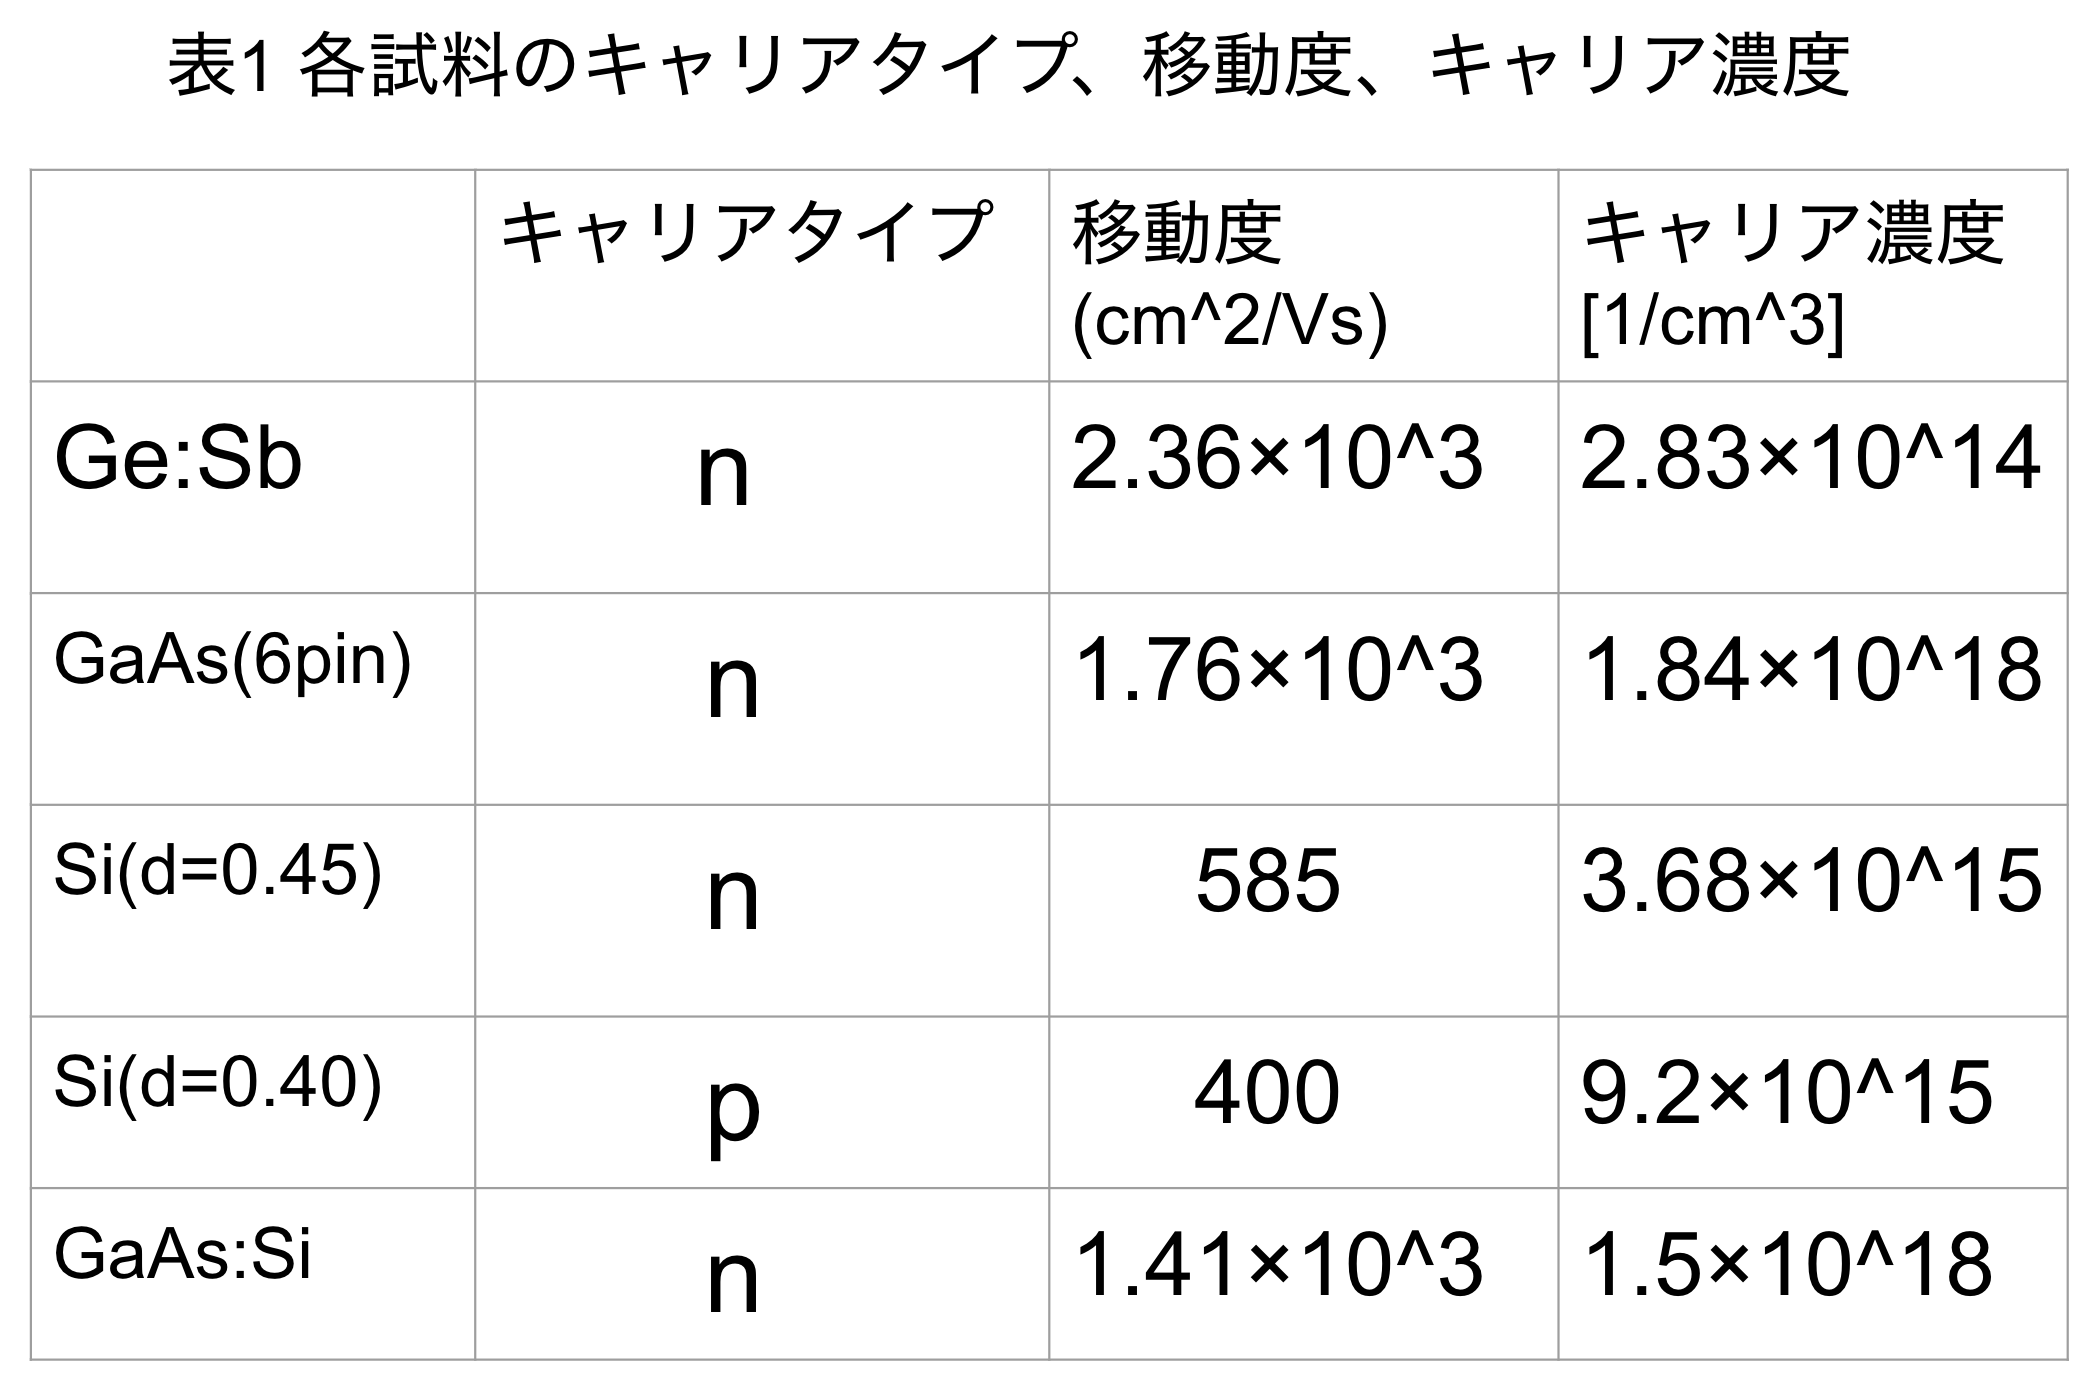
\includegraphics[scale = 0.4]{hyou.png}
\end{center}
\end{figure}

この表が各試料の測定結果のまとめである。キャリアタイプがnである方が移動度が大きい傾向がある。

\begin{figure}[H]
\begin{center}
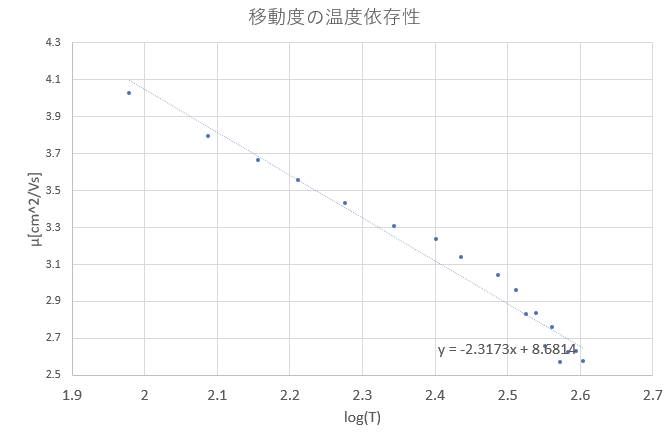
\includegraphics[scale = 1]{idoudo.png}
\caption{Ge試料の移動度の温度依存性}
\end{center}
\end{figure}
図9はGe試料の温度を変化させた時の移動度の変化である。$\log{T} = 2.5$を境に傾きが変化している。


\begin{figure}[H]
\begin{center}
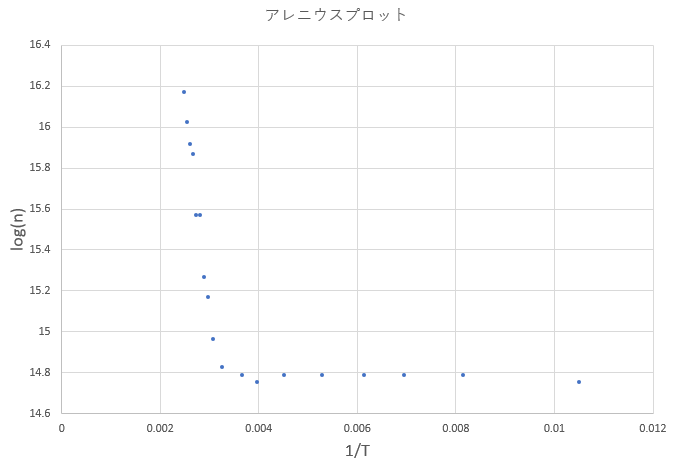
\includegraphics[scale = 1]{alenius.png}
\caption{Ge試料のキャリア濃度のアレニウスプロット}
\end{center}
\end{figure}

図10はGe試料のアレニウスプロットである。中央にはっきりと出払い領域が現れ、その左には真性領域、分かりづらいが右にフリーズアウト領域が確認できる。

\section{考察}
\subsection*{(1) 移動度}
移動度は、電界$E$中の、キャリアの平均速度$<v>$を用いて
\begin{equation}
\mu = \frac{<v>}{E}
\end{equation}
と定義される。

移動度を測定することにより、キャリアの結晶中での移動するときの通りやすさがわかる。
\subsection*{(2) 移動度の性質}
同種の半導体で、不純物濃度が同じなら、n型の方が移動度が大きい。
なぜなら、キャリアの電荷$q$と有効質量$m^{\ast}$に対し(15)式と等価な式
\begin{equation}
\mu = \frac{q\tau}{m^{\ast}}
\end{equation}が成り立ち、正孔より電子の方が有効質量が小さいからである。
\subsection*{(3) キャリア濃度の温度変化}
半導体のバンド構造で、不純物がドープされた半導体には、伝導帯の少し下にドナー準位が生じる。

・温度が中程度のとき、ドナー準位に存在していたキャリアは熱によって励起され伝導帯に移る。しかし価電子帯のキャリアは伝導帯、及びドナー準位にまでは励起されないので、キャリア濃度は一定となる。

・温度が低温になると、ドナー準位のキャリアが熱によって十分に励起されなくなり、全てのドナー準位のキャリアが伝導帯に移りきるまでは、温度が上昇するとともに、キャリア濃度も上昇していく。これをフリーズアウト現象と呼び、キャリア濃度$n$は、活性化エネルギーを$E_{d}$として、
\[n \propto \exp{(-\frac{E_{d}/2}{kT})}\]
と表される。

・温度が高温になると、価電子帯のキャリアが励起され、伝導帯に移るようになる。この温度に達すると、温度が上昇するとともに、伝導帯に移るキャリアが多くなり、キャリア濃度が大きくなっていく。

キャリア濃度は、バンドギャップエネルギーを$E_{G}$として、
\[n \propto \exp{(-\frac{E_{G}/2}{kT})}\]

と表される。

この式は、単位エネルギーあたりのキャリアの状態密度$n$、フェルミ-ディラックの分布関数$f(E)$を用いて、
\[n_{0} = \int _{0} ^{\infty} n(E)f(E)dE\]
として求まる。
$n(E) \propto \sqrt{E}, f(E) \propto \frac{1}{1+\exp{\left(\frac{E-\mu}{k_{0}T}\right)}} \sim \exp{\left(-\frac{E-\mu}{k_{0}T}\right)}$
と近似して積分を実行すると、
\[n_{0} = N_{C}\exp{\left(-\frac{E_{C}-E_{F}}{kT}\right)}\]
\[p_{0} = N_{V}\exp{\left(-\frac{E_{F}-E_{V}}{kT}\right)}\]
を得る。

これらをかけてルートをとることで、真性キャリア濃度が、
\[n_{i} \propto \exp{\left(-\frac{E_{G}}{2kT}\right)}\]
が得られる。
\subsection*{(4) アレニウスプロットの分析}
実験結果の、図10より、$1/T = 0.0032$、つまり$T = 310$Kほどで真性領域に達している。

一方、伝導体と価電子帯の実効状態密度を$N_{C}, N_{V}$とおくと、真性キャリア濃度$n_{i}$が
\begin{equation}
n_{i} = \sqrt{N_{C}N_{V}}\exp{\left(-\frac{E_{G}}{2kT}\right)}
\end{equation}
ただし、
\begin{equation}
N_{C} = 2\left(\frac{2\pi m_{e}kT}{h^{2}}\right)^{\frac{3}{2}}\\
, N_{V} = 2\left(\frac{2\pi m_{h}kT}{h^{2}}\right)^{\frac{3}{2}}
\end{equation}

理論式(17)に各値を代入し、アレニウスプロットのグラフを描画し、実験で得られたドナー濃度と等しくなる点を求めると、$1/T = 0.0029$すなわち、$T = 350K$ほどで出払い領域から、真性領域に達するという計算結果を得た。

ここで実験値と理論値が50Kほど異なっており10\% ほどの誤差があるが、実際は出払い領域と真性領域の境界ははっきりしていない、文献値と試料の値が異なるといったことが原因として考えられる。

バンドギャップは実験のアレニウスプロットの真性領域の傾きから求められた値が、0.70eV、一方で文献値が0.69eVであり、約1\% の誤差で一致している。
\subsection*{(5) 移動度の温度依存性}
実験(2)の結果図9から、
低温(100K周辺まで)ではおおよそ傾きが-1.8ほどになっていて音響フォノン散乱が支配的になっており、そこを超えるとさらに傾きが大きくなり、-2.3ほどになっていて、この領域では光学フォノン散乱が支配的となり、移動度を小さくしていると考えられる。

80K以下の領域で測定すると、温度の下降とともに移動度を下げる、イオンか不純物散乱が効き始め、80K付近が移動度のピークとなり、それとり低温の領域では移動度が小さくなっていくと考えられる。

\subsection*{(7) 半導体デバイスの活用}
CPU内のトランジスタを考えてみると、CPUは数GHzで動作するので、遅延なく動作するには、ドレイン電流が流れるために1nsでもかかってしまうと、CPUのクロックより遅くなり、CPUの動作を制限してしまう。移動度が大きいと、ドレイン電流が即座に流れて、CPUの動作を制限しない。

また、太陽電池において、高移動度の半導体デバイスを使えるようになると、大きくキャリアを拡散させることができ、性能を向上させることができる。

\subsection*{(9) パウ法の誤差}
パウ法では電極の接点が点だと仮定しているが、
実際の電極の接点は有限の大きさを持つので誤差が生じる。

また、実際は少し電極を端の内側に接続することになるので、仮定のように電極を試料の端に接続することもできないことが、誤差の一因となる。

\section{結論}

本実験を通して、半導体中のキャリアの振る舞いを定性的に、また定量的にも理解を深めることができた。

具体的にはホール効果によって、直接は測定することが難しい試料のキャリア濃度、移動度を間接的に測定し、移動度の意味、性質から、それらの温度依存性、活用までを考察し、深く理解することができた。

\section{参考文献}
[1]東京大学工学部:「電気電子情報実験・演習第二 テキスト 第2分冊」, 2019.

[2]柴田直:「半導体デバイス入門」, 数理工学社, 2014.

[3]岸野正剛:「半導体デバイスの基礎」, 丸善株式会社, 1995
\end{document}